\cotefile{156-9}
\scanpage{112}
\mspage{NA 20}
% archive sheet number: 111
% Typescript upside down in the scan; transcribed in its reading direction.
% One diagonal cancellation stroke crosses the entire body of the typescript.
% Nested deletion marks retain the separate local cancellations.
\deleted{(que je qualifie de ``foncteur de Mebkhout'' dans le texte) figurant dans la conjecture en question, m'a assuré son entière bonne foi, vu qu'il n'aurait pas eu connaissance de cet appendice à l'exposé de Ramis, avant que je ne lui communique la lettre de Schapira en faisant état, au mois de janvier dernier.}

\deleted{Page 951}

\deleted{($^{**}$) (6 mai 1986) C'est là du moins la ``version Mebkhout'' des choses, contredite par d'autres témoignages qui m'ont paru convainquants. Je n'ai pas de doute à présent que l'idée des foncteurs $m$ et $\unsure{M|\mathbb{M}}$ (formant la fameuse ``correspondance'' dite de Riemann-Hilbert), dans le cadre des catégories dérivées, est due à Kashiwara. \deleted{Mais \unsure{personnellement}, \unsure{jusqu'en décembre 1979},} cette conjecture \deleted{\unsure{a été regardée}} semble avoir été regardée, par ceux qui en avaient entendu parler tout comme par Kashiwara et Mebkhout, comme une curiosité mathématique sans grande conséquence, du moins jusqu' en septembre 1979.}

\deleted{Page 952}

\deleted{($^{*}$) (6 mai 1986) C'est là du moins la version Mebkhout, que j'avais prise pour argent comptant. J'en doute fortement à présent, et surtout (comme je le souligne dans de précédentes notes de bas de page, datées de ce jour) qu'il ait eu avant fin 1979 ou courant 1980 l'intuition du rôle crucial que cette équivalence de catégories (conjecturée d'abord par Kashiwara, selon toute apparence) allait avoir à jouer dans une nouvelle théorie de coefficients. Il convient donc de lire également avec un grain \deleted{\unsure{à}} de sel la note de b. de p. qui suit (du 5 mai l'an dernier).}

\deleted{Complément à la note de bas de page ($^{**}$)}

\deleted{($^{\unsure{x|\times}}$) (6 mai 1986) Pour une rectification au sujet de cette version, inexacte, voir les précisions datées de ce même jour, dans les notes de b. de p. ($^{*}$) p. 949 et ($^{*}$) p. 950: \deleted{\unsure{l'an dernier}} la conjecture pertinente est mentionnée dès janvier 1978 dans un texte de la plume de Ramis, qui l'attribue à Kashiwara.}

\deleted{Page 953}

\deleted{($^{*}$) (6 mai 1986) Pour des réserves vis-à-vis de cette terminologie ``foncteur de Mebkhout'', voir note de b. de p. ($^{\unsure{***|**}}$) p. 949. On pourrait peut-être aussi l'appeler ``foncteur de Kashiwara-Mebkhout'', vu le rôle important \deleted{\unsure{pris}} joué par Mebkhout, aussi bien pour faire réaliser son importance (via sa philosophie de dualité, notamment), que pour \unsure{le|la} \deleted{\unsure{l'immédiat}}}

% A small black mark below the last line has no recoverable letter shape.
\scanpage{113}
\mspage{107}
% archive sheet number: 112
% Pale mirrored typescript is show-through from the reverse, not text on this face.

\diagram{\begin{tikzcd}[ampersand replacement=\&,row sep=1.2em,column sep=1.1em]
 \& \& \& 1 \& \& \\
 \& \& \& \& A' \& \\
 B \& \& \& \& \& A \\
 \& \& \& C \& \& \\
 a \& \& c \& \& \& b' \\
 \& a' \& \& \& \& \\
 \& \& 0 \& \& \&
 \arrow[from=3-1,to=1-4]
 \arrow[from=4-4,to=1-4,very thick]
 \arrow[from=3-6,to=2-5]
 \arrow[from=2-5,to=1-4,very thick]
 \arrow[from=5-1,to=3-1]
 \arrow[from=5-1,to=4-4,very thick,"{\deleted{\unsure{b\prime|b|\beta}}}","{\unsure{\times}}"'{pos=0.25}]
 \arrow[from=5-3,to=3-1]
 \arrow[from=5-3,to=3-6,"{\deleted{\unsure{A}}}"{pos=0.75}]
 \arrow[from=5-3,to=4-4,very thick,"{\ast}","{\deleted{\unsure{a|\alpha}}}"']
 \arrow[from=5-6,to=4-4]
 \arrow[from=5-6,to=3-6]
 \arrow[from=7-3,to=6-2,very thick]
 \arrow[from=6-2,to=5-1]
 \arrow[from=7-3,to=5-3,very thick]
 \arrow[from=7-3,to=5-6]
\end{tikzcd}}

\figure{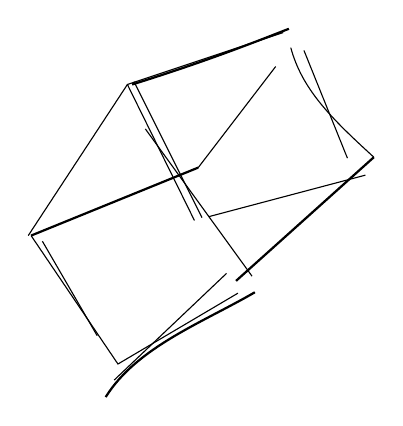
\begin{tikzpicture}[x=0.012cm,y=-0.012cm]
 \draw[thin] (990,545)--(1095,385)--(1260,330);
 \draw (1095,385)--(1166,529);
 \draw (1102,382)--(1174,526);
 \draw[thick] (1100,385).. controls (1180,360) and (1230,340)..(1266,326);
 \draw (1268,346).. controls (1280,390) and (1310,420)..(1356,462);
 \draw (1282,349)--(1328,463);
 \draw[thick] (1356,462)--(1210,593);
 \draw (1347,481)--(1181,525);
 \draw (1114,432)--(1227,588);
 \draw[thick] (993,545)--(1170,473);
 \draw (1170,473)--(1252,366);
 \draw (993,545)--(1085,681)--(1212,606);
 \draw (1005,551)--(1063,651);
 \draw[thick] (1072,716).. controls (1105,663) and (1175,637)..(1230,605);
 \draw (1081,698)--(1200,585);
\end{tikzpicture}}

\diagram{\begin{tikzcd}[ampersand replacement=\&,row sep=1.5em,column sep=2.5em]
 \& A \& \\
 c \& \& b \\
 B \& \& C \\
 \& a \&
 \arrow[from=2-1,to=1-2]
 \arrow[from=1-2,to=2-1,bend right=15,"{\unsure{\to|-}}"']
 \arrow[from=2-3,to=1-2]
 \arrow[from=1-2,to=2-3,bend left=25,"{\unsure{\to|-}}"]
 \arrow[from=2-1,to=3-1]
 \arrow[from=3-1,to=2-1,bend left=20]
 \arrow[from=2-3,to=3-3]
 \arrow[from=2-3,to=3-3,bend left=13,"{\unsure{\to|-}}"]
 \arrow[from=4-2,to=3-1]
 \arrow[from=4-2,to=3-1,bend left=15]
 \arrow[from=4-2,to=3-3]
 \arrow[from=4-2,to=3-3,bend right=12]
\end{tikzcd}}

\figure{\begin{tikzpicture}[x=1cm,y=1cm]
 \fill (0,0) circle (2pt) node[below=5pt] {$i$};
 \fill (.28,0) circle (2pt) node[below=5pt] {$i'$};
 \fill (1.8,-.06) circle (2pt) node[below=5pt] {$j$};
 \fill (4,-.12) circle (2pt) node[below=5pt] {$\unsure{h|k}$};
\end{tikzpicture}}

\[
\begin{aligned}
&\deleted{A\in I}\\
&\left\{E\in{\unsure{\mathscr{P}|\mathcal{P}|P}}^{3}(I)\ \middle|\
\begin{aligned}
i,i'\in E\quad&\text{ou}\quad j,i'\notin E\quad\text{ou}\\
E=\underbrace{\{i\}}_{a'}\quad&\text{ou}\quad E=\underbrace{\{i',j,k\}}_{A'}
\end{aligned}\right\}\\
&\deleted{\text{tel que}}
\end{aligned}
\]

\[
a',\ b,\ c,\qquad \unsure{b'|b}\vee c=A,\quad c\vee a'=B,\quad a'\vee b=C
\]

\diagram{\begin{tikzcd}[ampersand replacement=\&,row sep=.6em,column sep=3em]
 C\downarrow\deleted{\unsure{E|C|c}} \& C\downarrow \& C\downarrow \\
 a \& b\deleted{\unsure{\ast|a|\prime}} \& c \\
 \text{pas OK!} \& \text{OK} \& \text{OK}
\end{tikzcd}}
\scanpage{114}
\mspage{NA 27}
% archive sheet number: 113
% Typescript upside down in the scan; transcribed in its reading direction.

Page 1074

($^{**}$) (8 mai 1986) En écrivant ici ``du\deleted{\unsure{un}} cru de Kashiwara'', j'avais à l'esprit, bien sûr, l'incident au séminaire Goulaouic-Schwartz, telle que me l'avait rapporté Mebkhout. Je n'ai plus lieu de croire à présent qu'en cette occasion, Kashiwara ait agi de façon incorrecte, \deleted{\unsure{et pensé|et pense} que Mebkhout} Par contre, j'estime que d'autres actes d'appropriation du cru de Kashiwara et de certains de ses collaborateurs, dont il a été question par ailleurs, méritent bel et bien le nom d'``escroqueries''. J'avais pris soin d'ailleurs de faire parvenir à Kashiwara \deleted{dès} un exemplaire de ReS IV dès après tirage, suivi le 9 février dernier par une lettre d'excuses au sujet des déformations de la version Mebkhout, dont je m'étais fait l'écho\inserted{\handwritten{sans réserves}}. J'ai appris par ailleurs qu'il a reçu l'un et l'autre envoi. \deleted{\unsure{Il n'|Il m'}}\handwritten{\unsure{,}} Je n'ai reçu à ce jour aucun\deleted{\unsure{s}} signe de vie de lui, ni d'explication au sujet de\deleted{s} certains faits exposés dans Récoltes et Semailles le concernant, et qui ne peuvent guère faire l'objet \deleted{\unsure{d'un}}de doutes.

Page 1076

($^{*}$) (8 mai 1986) J'exprime ici vis-à-vis de Kashiwara un préjugé défavorable (à dire le moins) qui s'est avéré injustifié: la \unsure{vertité|vérité}, c'est que jusqu'en 1979 ou 1980, p e r s o n n e (me semble-t-il) \deleted{n'y} ne comprenait la place et la portée de ce résultat -- et Kashiwara, qui \deleted{\unsure{le|l'}}avait été le premier à le pressentir, ne le comprenait sans doute pas moins que les autres, y compris même peut-être Mebkhout lui-même. Après ``Verdier en personne'', j'ai supprimé ici la fin de la phrase\inserted{\handwritten{du texte original}}, encore plus désobligeante à l'encontre de Kashiwara que le début, et toute aussi abusive.

Page 1088

($^{*}$) (8 mai 1986) Je rappelle que c'est là la version de Mebkhout, qui à présent m'apparaît comme affabulatoire. Du coup, cela modifie de façon draconienne les présupposés ( m e s présupposés) dans l'incident au séminaire Goulaouic-Schwartz, dont il va être question. Les réflexions que cet incident m'avait inspirées l'an dernier ne m'en paraissent pourtant pas moins pertinentes. Et il n'y a aucun doute pour moi que l'avachissement et l'abdication de tous (ou du très grand nombre), devant la dégradation de l'éthique scientifique, est pour beaucoup dans l'exacerbation de dispositions conflictuelles à outrance, comme celles qui ont opposé Mebkhout à Kashiwara\deleted{\unsure{,}} et à d'autres.\deleted{\unsure{qu'il compte parmi les amis de celui}\illegible{1}}
\scanpage{115}
\mspage{10\deleted{\unsure{8}}9}
% archive sheet number: 114

Après cette longue \unsure{digression}, il faudrait revenir à l'axiome des supports dans un atelier.

\uline{Lemme} 1 Soit $\Sigma$ un \unsure{qtopos|topos}, $e_{\unsure{i|\ast|\bullet}}=(e_i)_{i\in I}$ une famille d'objets de $\Sigma$ mutuellement disjoints, \deleted{\unsure{Soit telle que}} non nuls, et telle que
\[
\deleted{\sum}\bigvee_i e_i=1_{\Sigma}.
\]

Conditions équivalentes

(i) \unsure{L'ens|L'un} des $e_i$ est contenu dans un sous ensemble $\deleted{\unsure{E}}\unsure{\mathbb{B}|B}_{\unsure{e|\alpha}}$ de $\Sigma$ stable pr \deleted{$\vee$, $\wedge$, $\unsure{\complement|C}$, et qui} $\operatorname{Sup}$, \deleted{et} $\operatorname{Inf}$ et $\complement$, et qui, pour la structure induite et l'unité, est une ``alg. de Boole''.

(ii) \deleted{L'ensemble} Pour tout $J\in\deleted{\unsure{I}}\inserted{\unsure{\mathscr{P}|\mathcal{P}|P}(I)}$, posons
\[
e_J=\operatorname{Sup}_{i\in J}\unsure{e_j|g|e_i}
\]
l'application ainsi obtenue
\[
\mathscr{P}(I)\unsure{\hookrightarrow|\longrightarrow}\Sigma\qquad J\longmapsto e_J
\]
% margin note written slanted
\margin{\uline{NB} Cette application est tjrs injective, car $J=\{i\in I\mid e_i\leq e_J\}$}
(qui commute \unsure{visiblement} aux $\operatorname{Sup}$ quelconques) commute à $\complement$ (donc aussi aux $\operatorname{Inf}$ quelconques).
\scanpage{116}
\mspage{110}
% archive sheet number: 115

Sous ces conditions, \deleted{$\unsure{B|\Sigma}$} l'image $\Sigma_e$ de cette application est le plus petit sous-ensemble $\Sigma'$ de $\Sigma$ satisfaisant les conditions de (i).

\uline{Cor 1} \unsure{Mêmes|Memes} \unsure{données|donnees}, mais on ne suppose pas que $e\overset{\mathrm{def}}{=}\operatorname{Sup}_{i\in I}e_i$ soit égal à $1$, et on introduit $e_0=\unsure{\complement|C}e$. Pour que les conditions du lemme soient satisfaites pour $\{\{e_i\},e_0\}$ (indexé pr $I\amalg\{0\}$) il f et s que \deleted{l'on ait,} pour tte partie $I'$ de $I$, posant $I''=I\setminus I'$, (de sorte que $e=e_{I'}\vee e_{I''}$, \deleted{on ait} $e_0=\complement e$), \deleted{on ait} \uline{on} ait
\[
\complement e_{I'}=e_{I''}\vee e_0
\]
ou ce qui revient au $=$ (\unsure{passant} aux $\complement$)
\[
e_{I'}=e\wedge\complement e_{I''}.
\]

\uline{Def} On dit alors que la \deleted{système}\inserted{famille} $(e_i)_{i\in I}$ d'éléments mutuellement disjoints est ``\uline{admissible}''. $\Sigma_{e_{\unsure{\ast|i|\bullet}}}=\Sigma_{(e_i)}$, alg. de Boole \unsure{engendrée}, \unsure{is.|iso.} à $\unsure{\mathscr{P}|\mathcal{P}|P}(I\amalg\{e_0\})$.
\scanpage{117}
\mspage{111}
% archive sheet number: 116

Ainsi, le premier axiome sur les supports dans un atelier, muni d'un magasin \deleted{\unsure{adjoint}}\inserted{associé} $\unsure{\mathscr{F}|\mathcal{F}|F}$, sera

\uline{Axiome supp 1} Pour toute figure $F\in\mathscr{F}_{c}$\inserted{$\operatorname{Figat}(\unsure{\mathcal{A}|\mathscr{A}|\mathbb{A}})$}, la famille des $(X^{\unsure{\circ|0|o}})_{X\in F}$ de $\Sigma_{\mathcal{A}}$ est admissible.

Cet axiome n'est pas \unsure{redondant}; comme on voit en \unsure{partant} d'un \unsure{qtopos|topos} $\Sigma$, et en prenant l'atelier $\operatorname{Figel}\overset{\deleted{\mathrm{fin}}}{\operatorname{spat}}_{\mathrm{fin}}(\Sigma)$, \deleted{et} des figures élémentaires\inserted{spatiales} finies (disons) de $\Sigma$, et le magasin \deleted{des} associé $\operatorname{Fig}\deleted{\mathrm{el}}\operatorname{spat}_{\mathrm{fin}}(\Sigma)$ des figures spatiales finies. La validité de l'axiome des supports revient alors, d'après le cor. 1, à ceci
\[
\left\vert\begin{aligned}
&\text{si }e,e'\in\Sigma\text{ avec }e\mid\unsure{0|o}\mid e',\quad
\deleted{\text{et si }e''=\unsure{\complement|C}e\vee e',}\\
&\deleted{\text{alors}}\ \text{alors }e'=(\complement e)\wedge(e\vee e').
\end{aligned}\right.
\]
Ou encore, la validité des conditions du lemme 2 (p. 105) sur $\Sigma$.
\scanpage{118}
\mspage{112}
% archive sheet number: 117

L'axiome des supports ne concerne directement que les données $\unlhd$, $|\unsure{0|o}|$ et $\unsure{\mathscr{F}|\mathcal{F}|F}\subset\unsure{\mathscr{P}|\mathcal{P}|P}(\unsure{\mathcal{A}|\mathscr{A}|\mathbb{A}})$ sur $A$, et ne fait pas intervenir encore $\overset{\circ}{\ll}$ ou $\ll$. Je \unsure{convient|conviens} de le renforcer ainsi.

Considérons dans un \unsure{qtopos|topos} $\Sigma$ toutes les \deleted{familles $(e_{\ast},I)=(e_i)_{i\in I}$}\inserted{parties} \deleted{$e_{\ast}=\{e_i\}_{i\in\unsure{J|I}}$} $A$, finies d'objets \deleted{\unsure{non}} nuls mutuellement disjoints. On peut les considérer comme des objets de $\operatorname{Figspat}(\Sigma)$, pour la relation d'ordre discret (disons) sur $\deleted{\unsure{\Sigma|e_{\ast}}}A$. Nous allons écrire, pour
\[
A,B\in\operatorname{Figspatdisc}(\Sigma),
\]
\[
\deleted{\unsure{A}}B\ll\deleted{\unsure{B}}A\quad\Longleftrightarrow\quad
\forall\deleted{\unsure{a}}b\in\deleted{\unsure{A}}B,\quad
\exists\deleted{\unsure{b}}a\in\deleted{\unsure{B}}A\text{ avec }b\leq a
\]
(\uline{NB} c'est aussi la relation \inserted{induite par} $\ll$ de $\operatorname{Figspat}$)

\deleted{Car} Pour un $\deleted{\unsure{b}}a\in\deleted{\unsure{B}}A$ donné, considérons l'ens $\deleted{\unsure{A_b}}B_a=\{b\in\deleted{\unsure{A}}B\mid b\leq a\}$, formé des éléments de $\deleted{\unsure{A}}B$ (mut. disj.) qui sont $\leq a$. Soit $\deleted{\unsure{b'}}a'=\operatorname{Sup}\deleted{\unsure{A_b}}B_a\leq\deleted{\unsure{b}}a$, et $\deleted{\unsure{b''}}a''=b\wedge\unsure{\complement|C}b'$.
